\documentclass[aspectratio=169]{beamer}
\setbeamertemplate{footline}[frame number]
%\documentclass[aspectratio=169,notes=only]{beamer}
\usepackage{multicol}
\usepackage{wrapfig}
\usepackage{algorithmicx}
\usepackage{algpseudocode}
\usepackage{graphicx}
%\usepackage{subcaption} % cannot be used

\usepackage[english]{layout}
\usepackage[utf8]{inputenc}
\usepackage[english]{babel}
\usepackage[T1]{fontenc}
\usepackage{amsmath, soul, color, multicol, type1cm, verbatim, latexsym, dsfont, float, listings,alltt,tikz, lmodern, textcomp}
\usepackage[official]{eurosym}
\usepackage[export]{adjustbox}
\usepackage[caption = false]{subfig}
%\usepackage{beamerthemesplit}
%\usetheme{Frankfurt}
\usecolortheme{lily}
%\usefonttheme{structuresmallcapsserif}
\usefonttheme{professionalfonts}
\setbeamercovered{transparent}

\newcommand{\pluseq}{\mathrel{{+}{=}}}

%NeSI Colors <-------------------------------------------------------------------------------------
\usecolortheme{lily}
\usecolortheme[RGB={47, 68, 71}]{structure} 
\definecolor{nesidark}{HTML}{2F4447}
\definecolor{nesilight}{HTML}{CED9DF}
\definecolor{nesigrey}{gray}{0.7}
\definecolor{nesilightgrey}{gray}{0.98}
\definecolor{nesidarkgrey}{gray}{0.3}
\definecolor{nesiblue}{HTML}{2B9FC2}
\setbeamercolor{block title}{fg=black,bg=nesigrey}
\setbeamercolor{block body}{bg=nesilightgrey,fg=nesidarkgrey}
\setbeamercolor{block body alerted}{bg=white,fg=black}
\setbeamercolor{alerted text}{bg=white,fg=black}
\addtobeamertemplate{frametitle}{\vskip+1.2ex}{}
%NeSI Custom Code Hightlight <---------------------------------------------------------------------------------------
\lstdefinestyle{customcode}{
  belowcaptionskip=1\baselineskip,
  breaklines=true,
  xleftmargin=\parindent,
  showstringspaces=false,
  basicstyle=\ttfamily,
  keywordstyle=\bfseries\color{green!40!black},
  commentstyle=\itshape\color{purple!40!black},
  identifierstyle=\color{blue},
  stringstyle=\color{orange},
}
%NeSI Title <---------------------------------------------------------------------------------------
\setbeamerfont{title}{size=\huge}
\frenchspacing
\hyphenation{NeSI}
%NeSI Template parameters <-------------------------------------------------------------------------
\setbeamertemplate{blocks}[default]
\useinnertheme{circles}
\setbeamertemplate{title page}[default][center,rounded=false,shadow=false]
\newcommand\BackgroundPicture[1]{%
\setbeamertemplate{background}{%
\parbox[c][\paperheight]{\paperwidth}{%
\vfill \hfill \includegraphics[height=\paperheight]{#1}
\hfill \vfill
}}}

%\pagenumbering{arabic}

%Content Starts Here <-------------------------------------------------------------------------------
\title{\LARGE{Two interpolation methods for vector fields that conseve flux and line integrals}}
%\subtitle{Computational Science team}
\author{Alexander Pletzer (NeSI/NIWA) and Wolfgang Hayek (NIWA/NeSI)\\
(alexander.pletzer@nesi.org.nz) \\
 C3DIS, Canberra\\
 7 May 2019  }
\date{}

\begin{document}
\BackgroundPicture{NeSI/title.png}
\begin{frame}[plain]
  \vspace{+1.0cm}
  \titlepage
\end{frame}

% This will generate the outline. If you have several topics, uncomment the multicols 
\BackgroundPicture{NeSI/blank-01.png}

%%%%%%%%%%%%%%%%%%%%%%%%%%%%%%%%%%%%%%%%%%%%%%%%%%%%%%%%%%%%%%%%%%%%%%%%%%%%%%%%%%%%%%%%%%%%%%%
%%%%%%%%%%%%%%%%%%%%%%%%%%%%%%%%%%%%%%%% Some Examples %%%%%%%%%%%%%%%%%%%%%%%%%%%%%%%%%%%%%%%%
%%%%%%%%%%%%%%%%%%%%%%%%%%%%%%%%%%%%%%%%%%%%%%%%%%%%%%%%%%%%%%%%%%%%%%%%%%%%%%%%%%%%%%%%%%%%%%%
% List with bullets (itemize) <---
% The [<+-| alert@+>] will create a new slide for each element with highlighting 


\BackgroundPicture{NeSI/divider-01.png}
\begin{frame}[fragile]{}
  \begin{center}
    \Huge{\textbf{Motivation}}
  \end{center}
\end{frame}
\BackgroundPicture{NeSI/blank-01.png}

\begin{frame}[t]
  \frametitle{Want answers to following questions}
    \begin{block}{How should we interpolate vector fields with staggered components?}
      \begin{itemize}%[<+-| alert@+>]
	  \item Arakawa C/D grids
      \item Components are on cell faces or edges
      \item Arises in computational fluid dynamics and electromagnetics
    \end{itemize}
  \end{block}
  \begin{tabular}{lr}
      % after \\: \hline or \cline{col1-col2} \cline{col3-col4} ...
      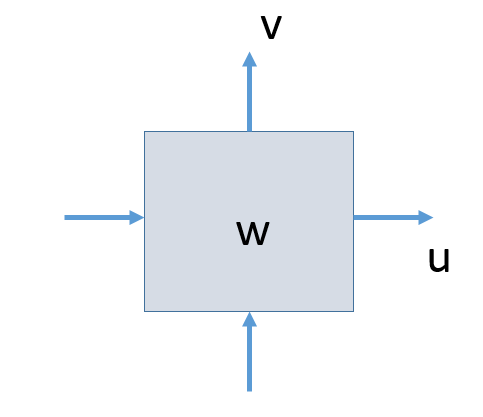
\includegraphics[width=30mm]{uvArakawaC.PNG} &               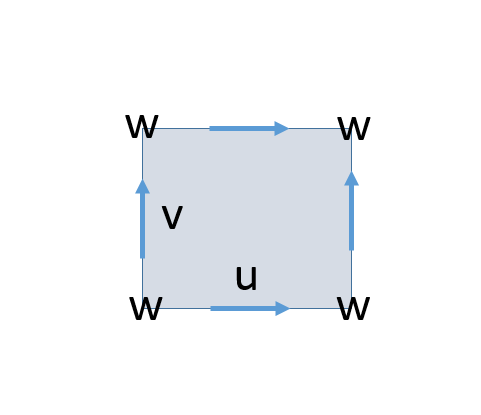
\includegraphics[width=30mm]{uvArakawaD.PNG} \\
      {Arakawa C-grid} & {Arakawa D-grid}  
\end{tabular}
\end{frame}

\begin{frame}[t]
  \frametitle{}
    \begin{block}{Can we unify existing interpolation methods?}
      \begin{itemize}%[<+-| alert@+>]
	  \item Linear, used since Babylonian times (2000-1700 BC)
      \item Conservative or area weighted, used in climate studies to enforce conservation
      \item In both cases the interpolation weights are ratios of areas (volumes)
      \item Should vector fields with staggered components use bilinear or conservative? Or something else?
    \end{itemize}
  \end{block}
  \begin{tabular}{lr}
      % after \\: \hline or \cline{col1-col2} \cline{col3-col4} ...
      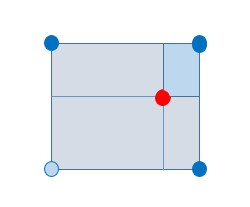
\includegraphics[width=30mm]{bilinear.png} &               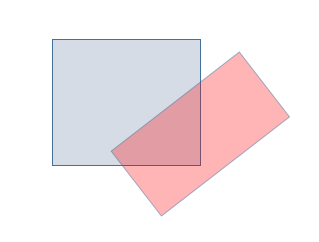
\includegraphics[width=30mm]{conservative.png} \\
      {Bilinear} & {Conservative}  
\end{tabular}
\end{frame}

\begin{frame}[t]
  \frametitle{}
  \begin{block}{How to handle curvilinear grids with non-orthogonal cells?}
  \end{block}
    Example: cubed-sphere grid
    \begin{itemize}
      \item Project grids on the surface of a cube onto a sphere
      \item Six logically rectangular grids (cannot be represented as a single structured grid)
      \item No pole-like singularity but some distortion where three tiles meet 
    \end{itemize}
  \begin{center}
    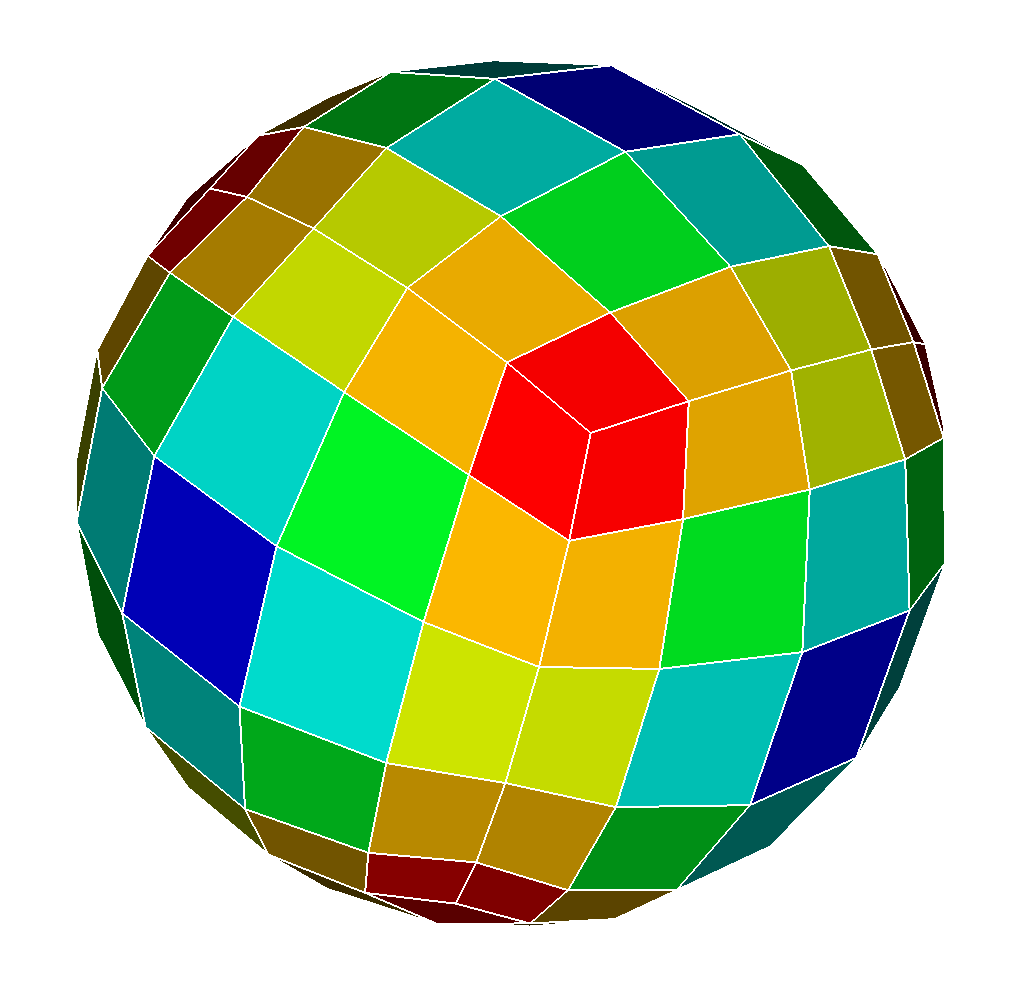
\includegraphics[width=0.35\textwidth]{cubedSphere.png}
  \end{center}
\end{frame}

\begin{frame}[t]
  \frametitle{}
  \begin{block}{How to compute surface fluxes?}
  \end{block}
  For example compute water fluxes across area
  \begin{center}
    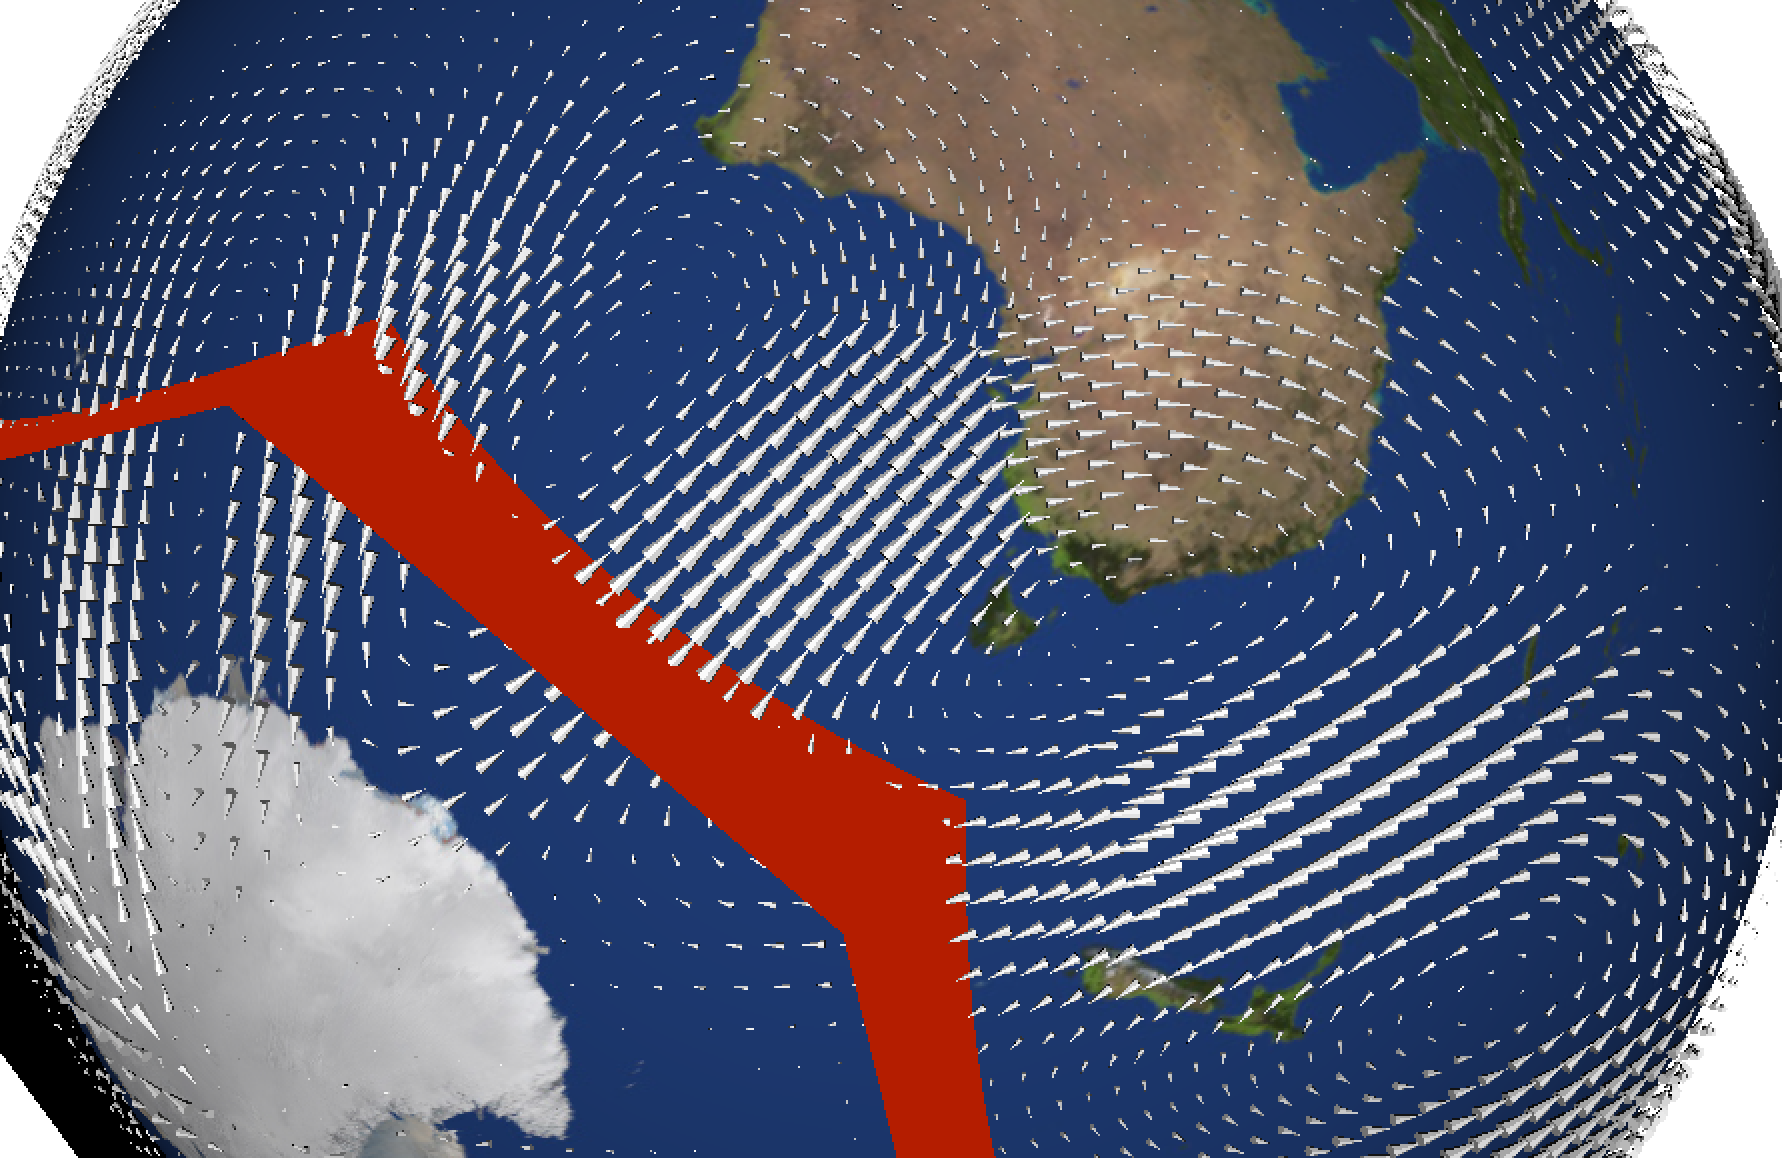
\includegraphics[width=0.6\textwidth]{fluxIntegral.png}
  \end{center}
  
\end{frame}

%\subsection{Divider examples}
\BackgroundPicture{NeSI/divider-02.png}
\begin{frame}[fragile]{}
  \begin{center}
    \Huge{\textbf{The type of field determines the discretization}}
  \end{center}
\end{frame}
\BackgroundPicture{NeSI/blank-01.png}

\begin{frame}[t]
  \frametitle{Why four types of fields?}
    \begin{block}{One derivative - 4 fields }
      \begin{itemize}%[<+-| alert@+>]
	  \item {\color{red} 0-form}: just a function of space, one component
        \begin{itemize}
          \item invariant under coordinate change
          \item Example: temperature
        \end{itemize}
      \item {\color{red} 1-form}: vector field, 3 components in 3D
        \begin{itemize}
          \item Examples: electric field $E$ and induction $H$
        \end{itemize}
      \item {\color{red} 2-form}: pseudo-vector field, 3 components in 3D
         \begin{itemize}
          \item Examples: magnetic field $B$ and displacement field $D$
        \end{itemize}
   \item {\color{red} 3-form}: pseudo-scalar, 1 component
         \begin{itemize}
          \item Example: density
        \end{itemize}
    \end{itemize}
  \end{block}
\end{frame}

\begin{frame}[t]
  \frametitle{Discretized versions of the fields}
    \begin{block}{Association of form with cell elements}
      \begin{itemize}%[<+-| alert@+>]
	  \item 0-form: {\color{red} on nodes}
        \begin{itemize}
          \item $\int \alpha = \alpha$ (integral is a no op)
        \end{itemize}
      \item 1-form: {\color{red} on edges}
        \begin{itemize}
          \item $\int \beta$ is a line integral
        \end{itemize}
      \item 2-form: {\color{red} on faces}
        \begin{itemize}
          \item $\int \gamma$ is a surface integral
        \end{itemize}
      \item 3-form: {\color{red} cell centred}
        \begin{itemize}
          \item $\int \omega$ is a volume integral
        \end{itemize}
    \end{itemize}
  \end{block}
  \begin{block}{Differential forms like to be integrated}
  \end{block}
\end{frame}

%\subsection{Divider examples}
\BackgroundPicture{NeSI/divider-04.png}
\begin{frame}[fragile]{}
  \begin{center}
    \Huge{\textbf{Interpolation}}
  \end{center}
\end{frame}
\BackgroundPicture{NeSI/blank-01.png}

\begin{frame}[fragile]{Generalizing ``interpolation''}
\begin{block}{Making interpolation work for nodal, edge, face and cell fields}
$\int f = \sum_i f_i \int_T \phi_i$
\begin{itemize}
\item $\phi_i$ is basis $k$-form, $k =$ 0, 1, 2 or 3
\item $T$ is target (point, line, area or volume)
\item $f_i$ is field integral over cell element $k$ (node, edge, face or cell)
\item $\int_T \phi_i$ is the interpolation weight
\item $i$ index runs over all the degrees of freedom (points, edges, faces etc., as appropriate)
\end{itemize}
\end{block}
\end{frame}

\begin{frame}[fragile]{Want the basis functions to satisfy orthogonality condition}

\begin{block}{$\int_i \phi_j = \delta_{ij}$}
 \begin{itemize}
   \item $i$ is cell element (node, edge, face, cell)
   \item $j$ is basis function index
   \item nodal bases are zero on all nodes expect one where it is one
   \item edge bases have zero integral on all edges except itself where it is one
   \item face bases have zero integral on all faces except itself where it is one
 \end{itemize}
 \end{block}

\end{frame}


\begin{frame}[fragile]{Observe how the $k = 1, 2$ bases satisfy the orthogonality condition}

  \begin{tabular}{lr}
      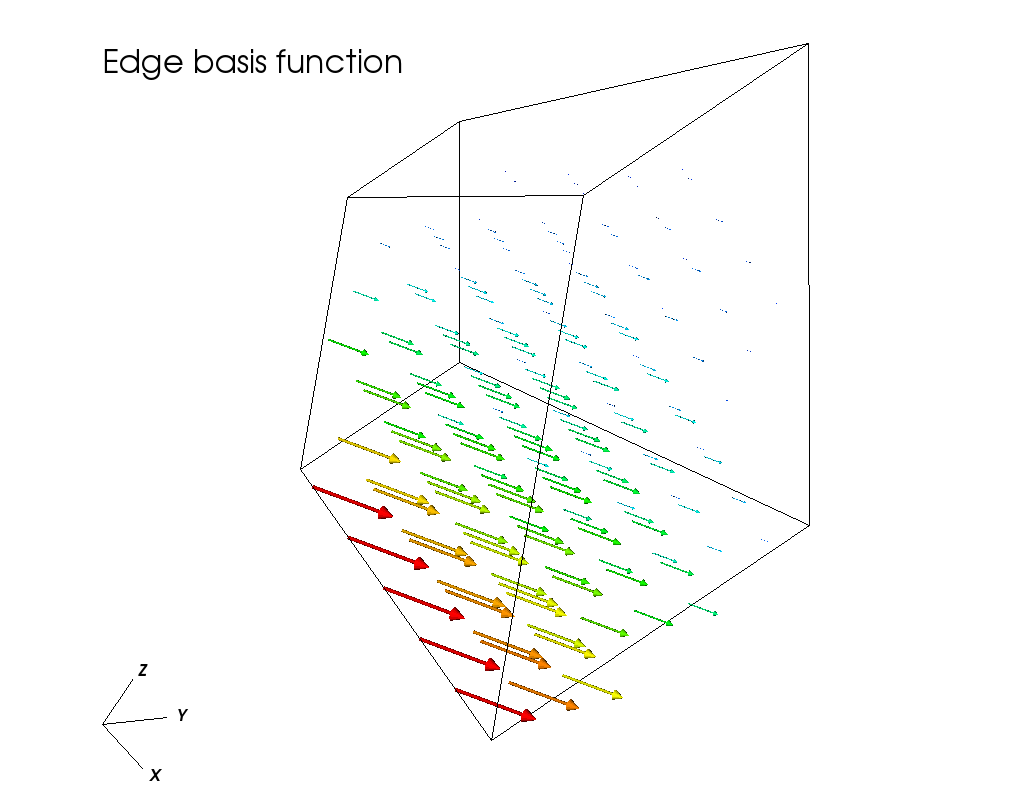
\includegraphics[width=50mm]{hexEdge.png} &                        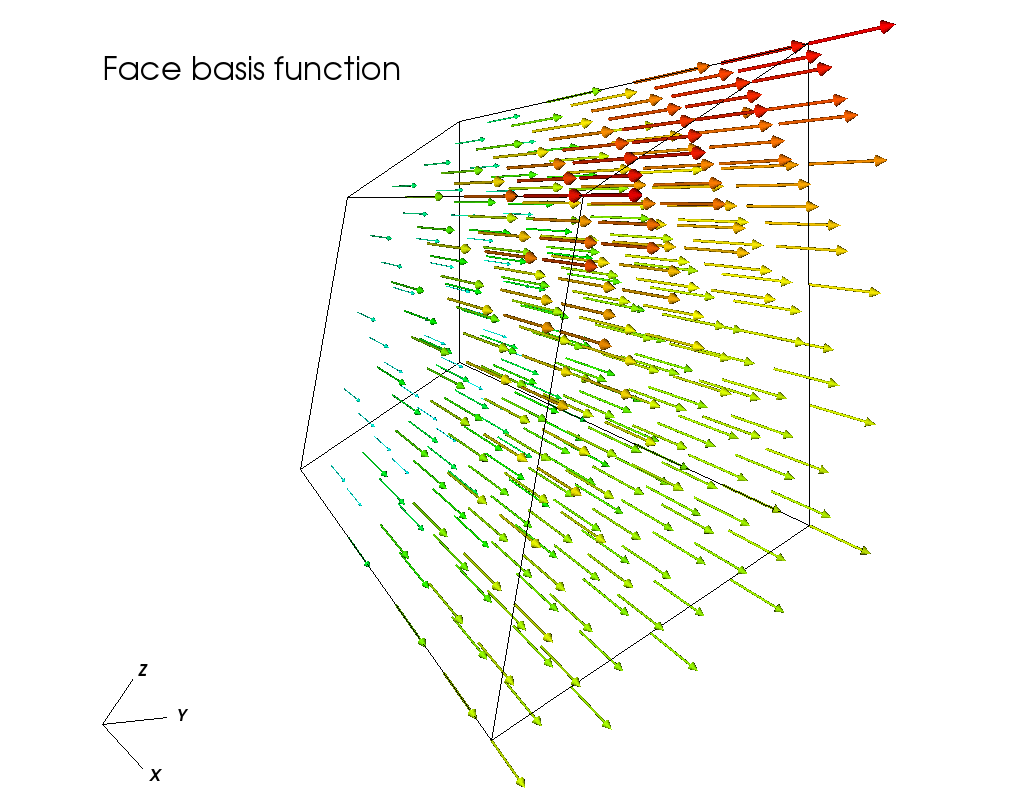
\includegraphics[width=50mm]{hexFace.png} \\
      {Edge basis is perpendicular } & {Face basis is tangent }  \\
      {to neighbouring edges} & {to neighbouring faces}
\end{tabular}


%\centering
%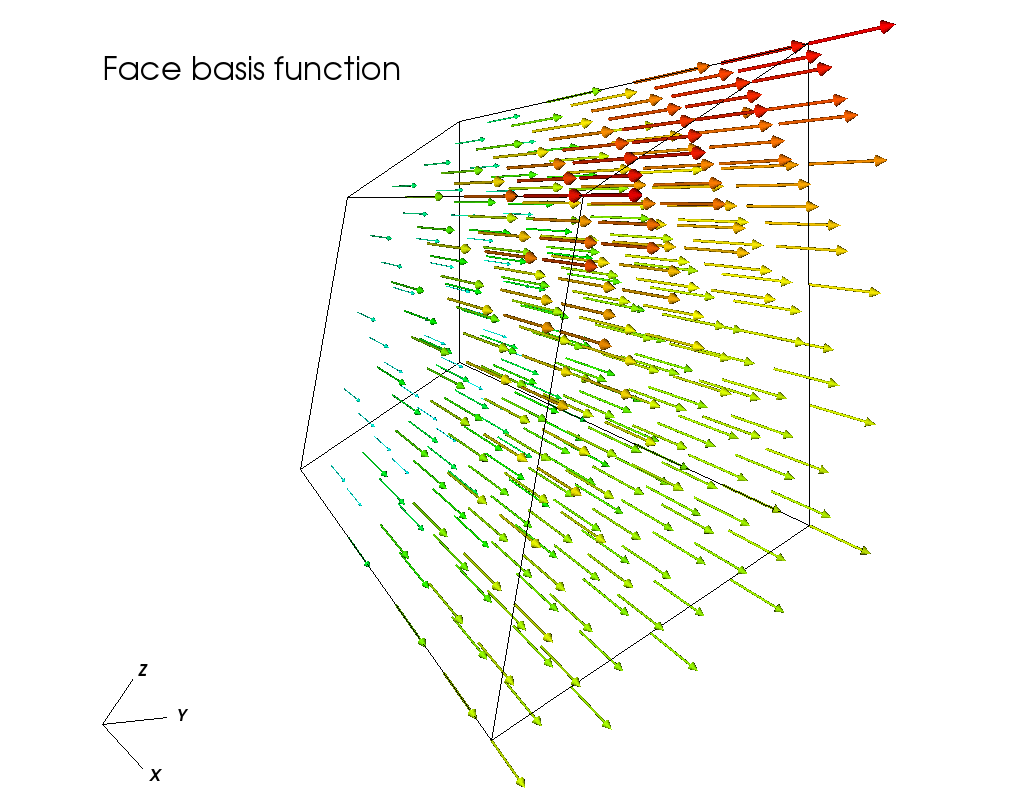
\includegraphics[width=0.3\textwidth]{hexFace.png}
% 2-form basis vanishes on opposite face and is tangent to incident faces
% \end{block}
\end{frame}

%\subsection{Divider examples}
\BackgroundPicture{NeSI/divider-04.png}
\begin{frame}[fragile]{}
  \begin{center}
    \Huge{\textbf{Results}}
  \end{center}
\end{frame}
\BackgroundPicture{NeSI/blank-01.png}

\begin{frame}[t]
  \frametitle{Divergence-free field in Cartesian coordinates}
  \begin{block}{Flux integral depends only on distance of endpoints to nearest grid node}
  \end{block}
  \begin{itemize}
  \item $v = dz \wedge d\psi$
  with stream function $\psi = \frac{\cos 2 \pi x}{4 \pi} + y^2$
  \item Closed surface fluxes $B$ and $C$ are exact 
  \end{itemize}
  \begin{center}
    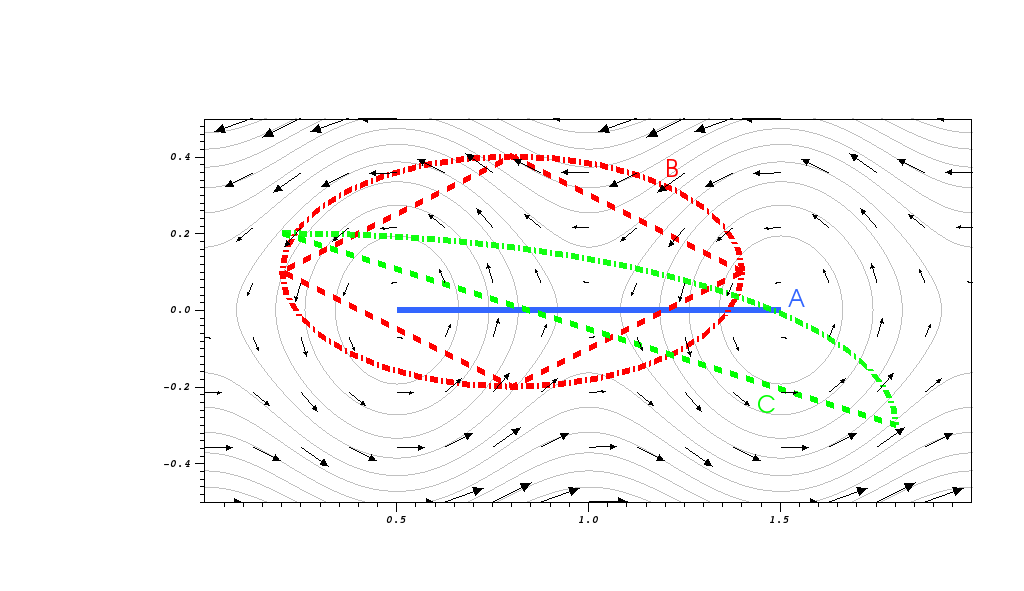
\includegraphics[width=.7\linewidth]{flow.png}
  \end{center}
\end{frame}

\begin{frame}[t]
  \frametitle{Vector field with singularity}
  \begin{block}{Numerical loop integral A gives 0, B gives 1}
   $v = \frac{x dx + y dy}{2 \pi (x^2 + y^2)}$
  \end{block}
  \begin{center}
    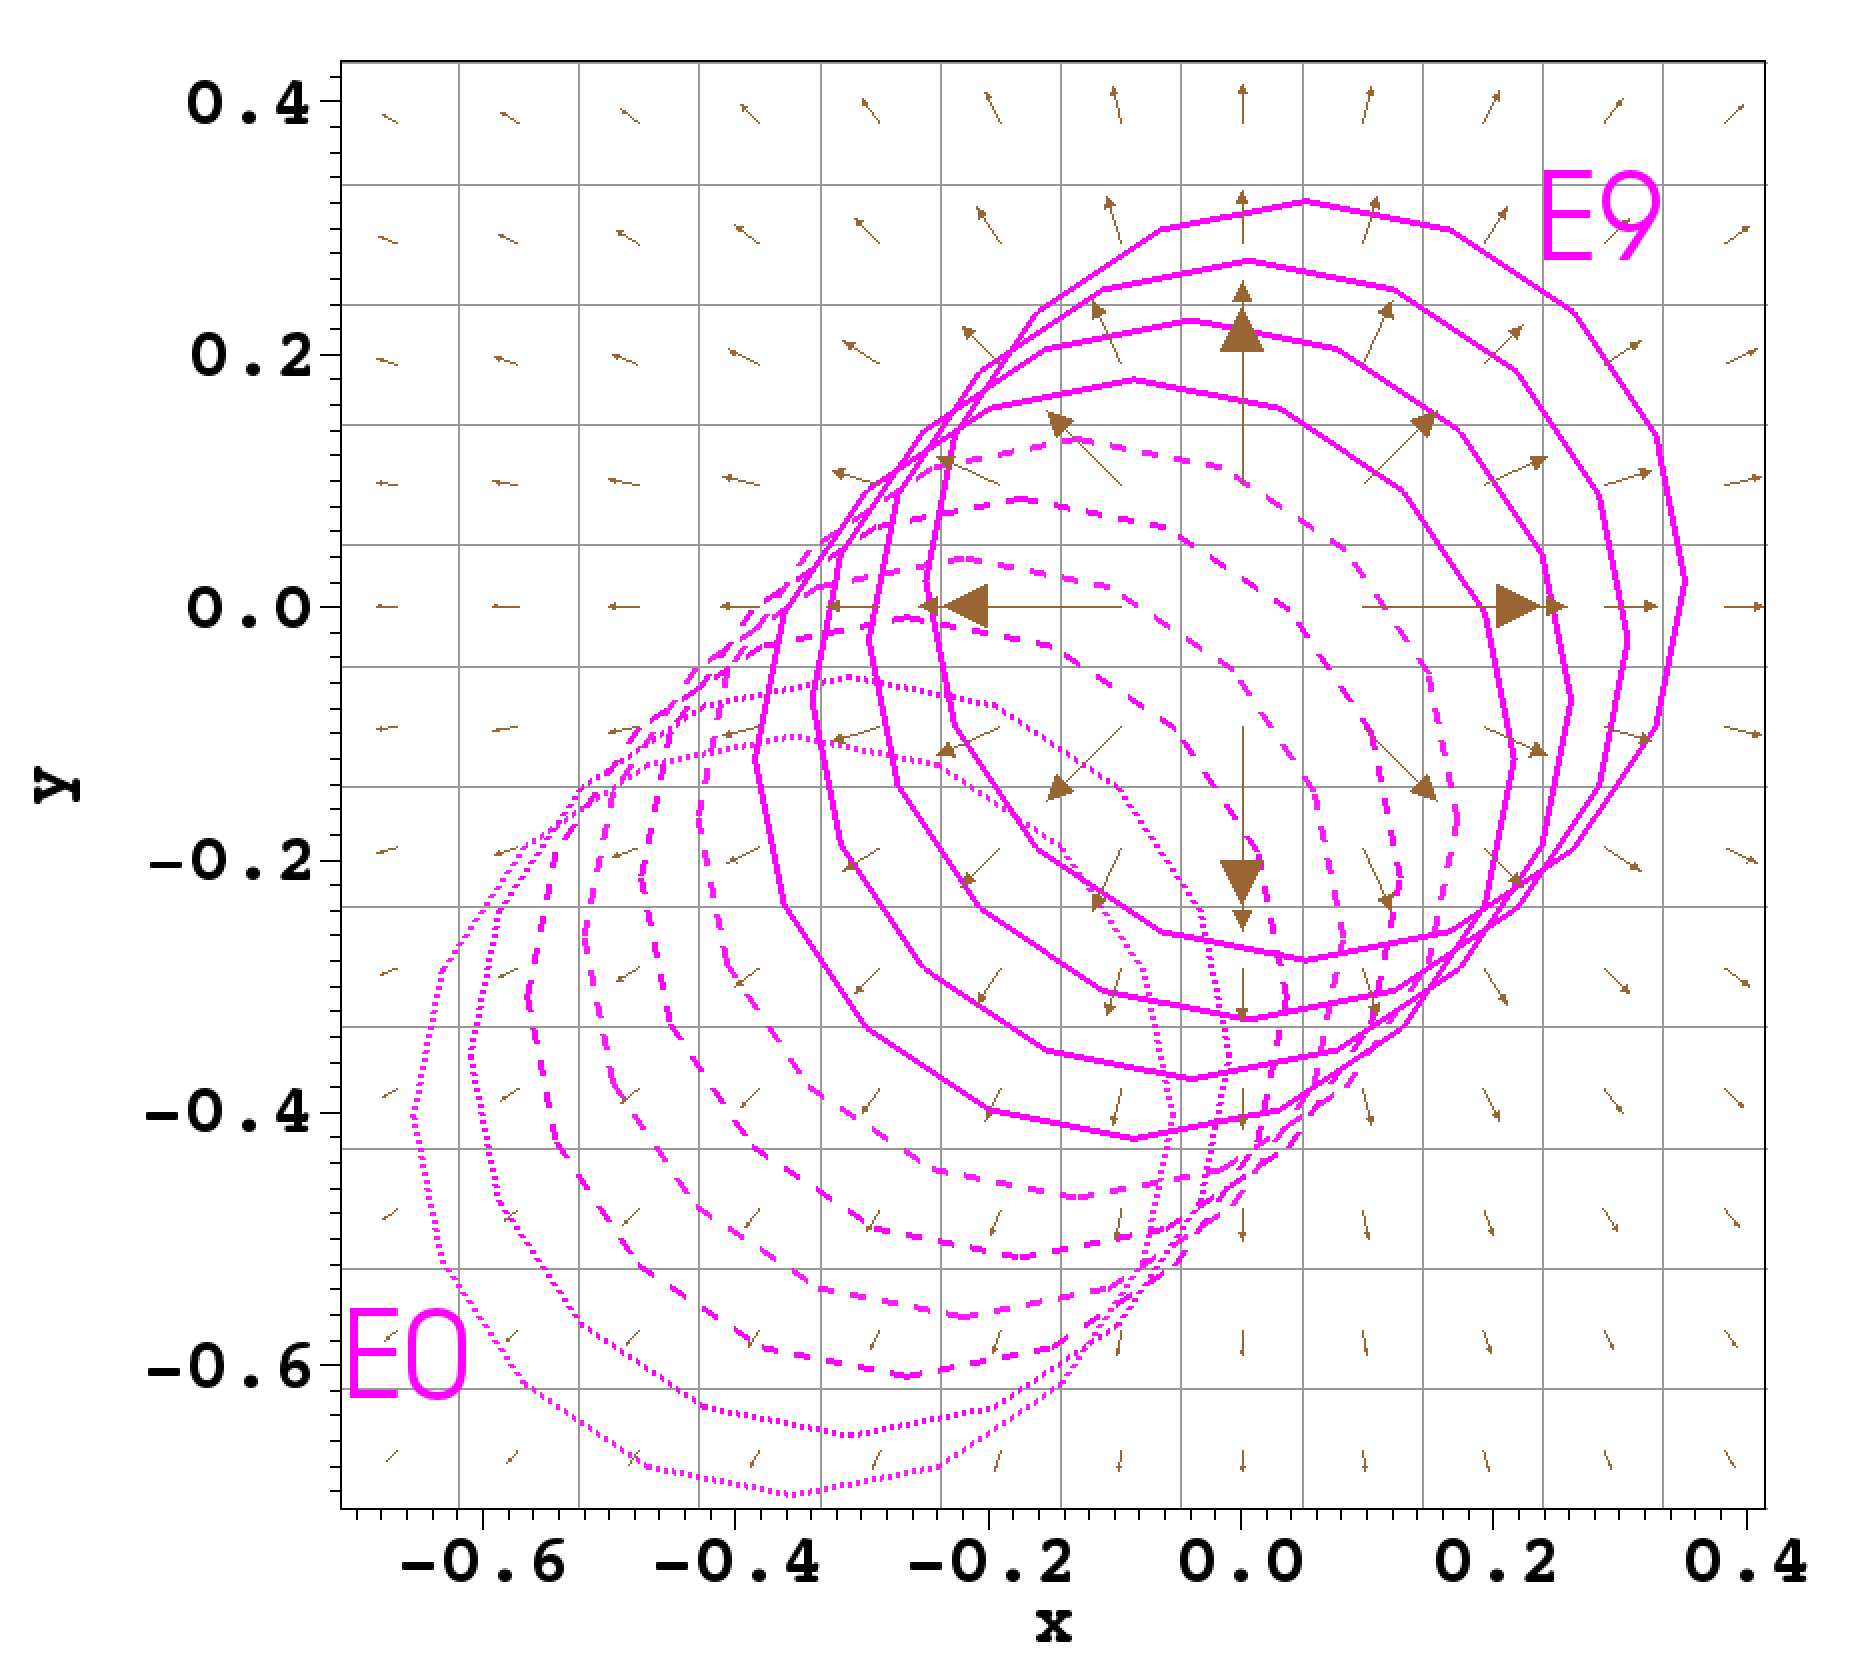
\includegraphics[width=.5\linewidth]{polar.png}
  \end{center}
\end{frame}

\begin{frame}[t]
  \frametitle{Flux computation on the cubed sphere $v = d\psi \wedge dr$}
  \begin{block}{Mimetic interpolation works for highly distorted cells}
  \end{block}
  
  \begin{tabular}{lr}
  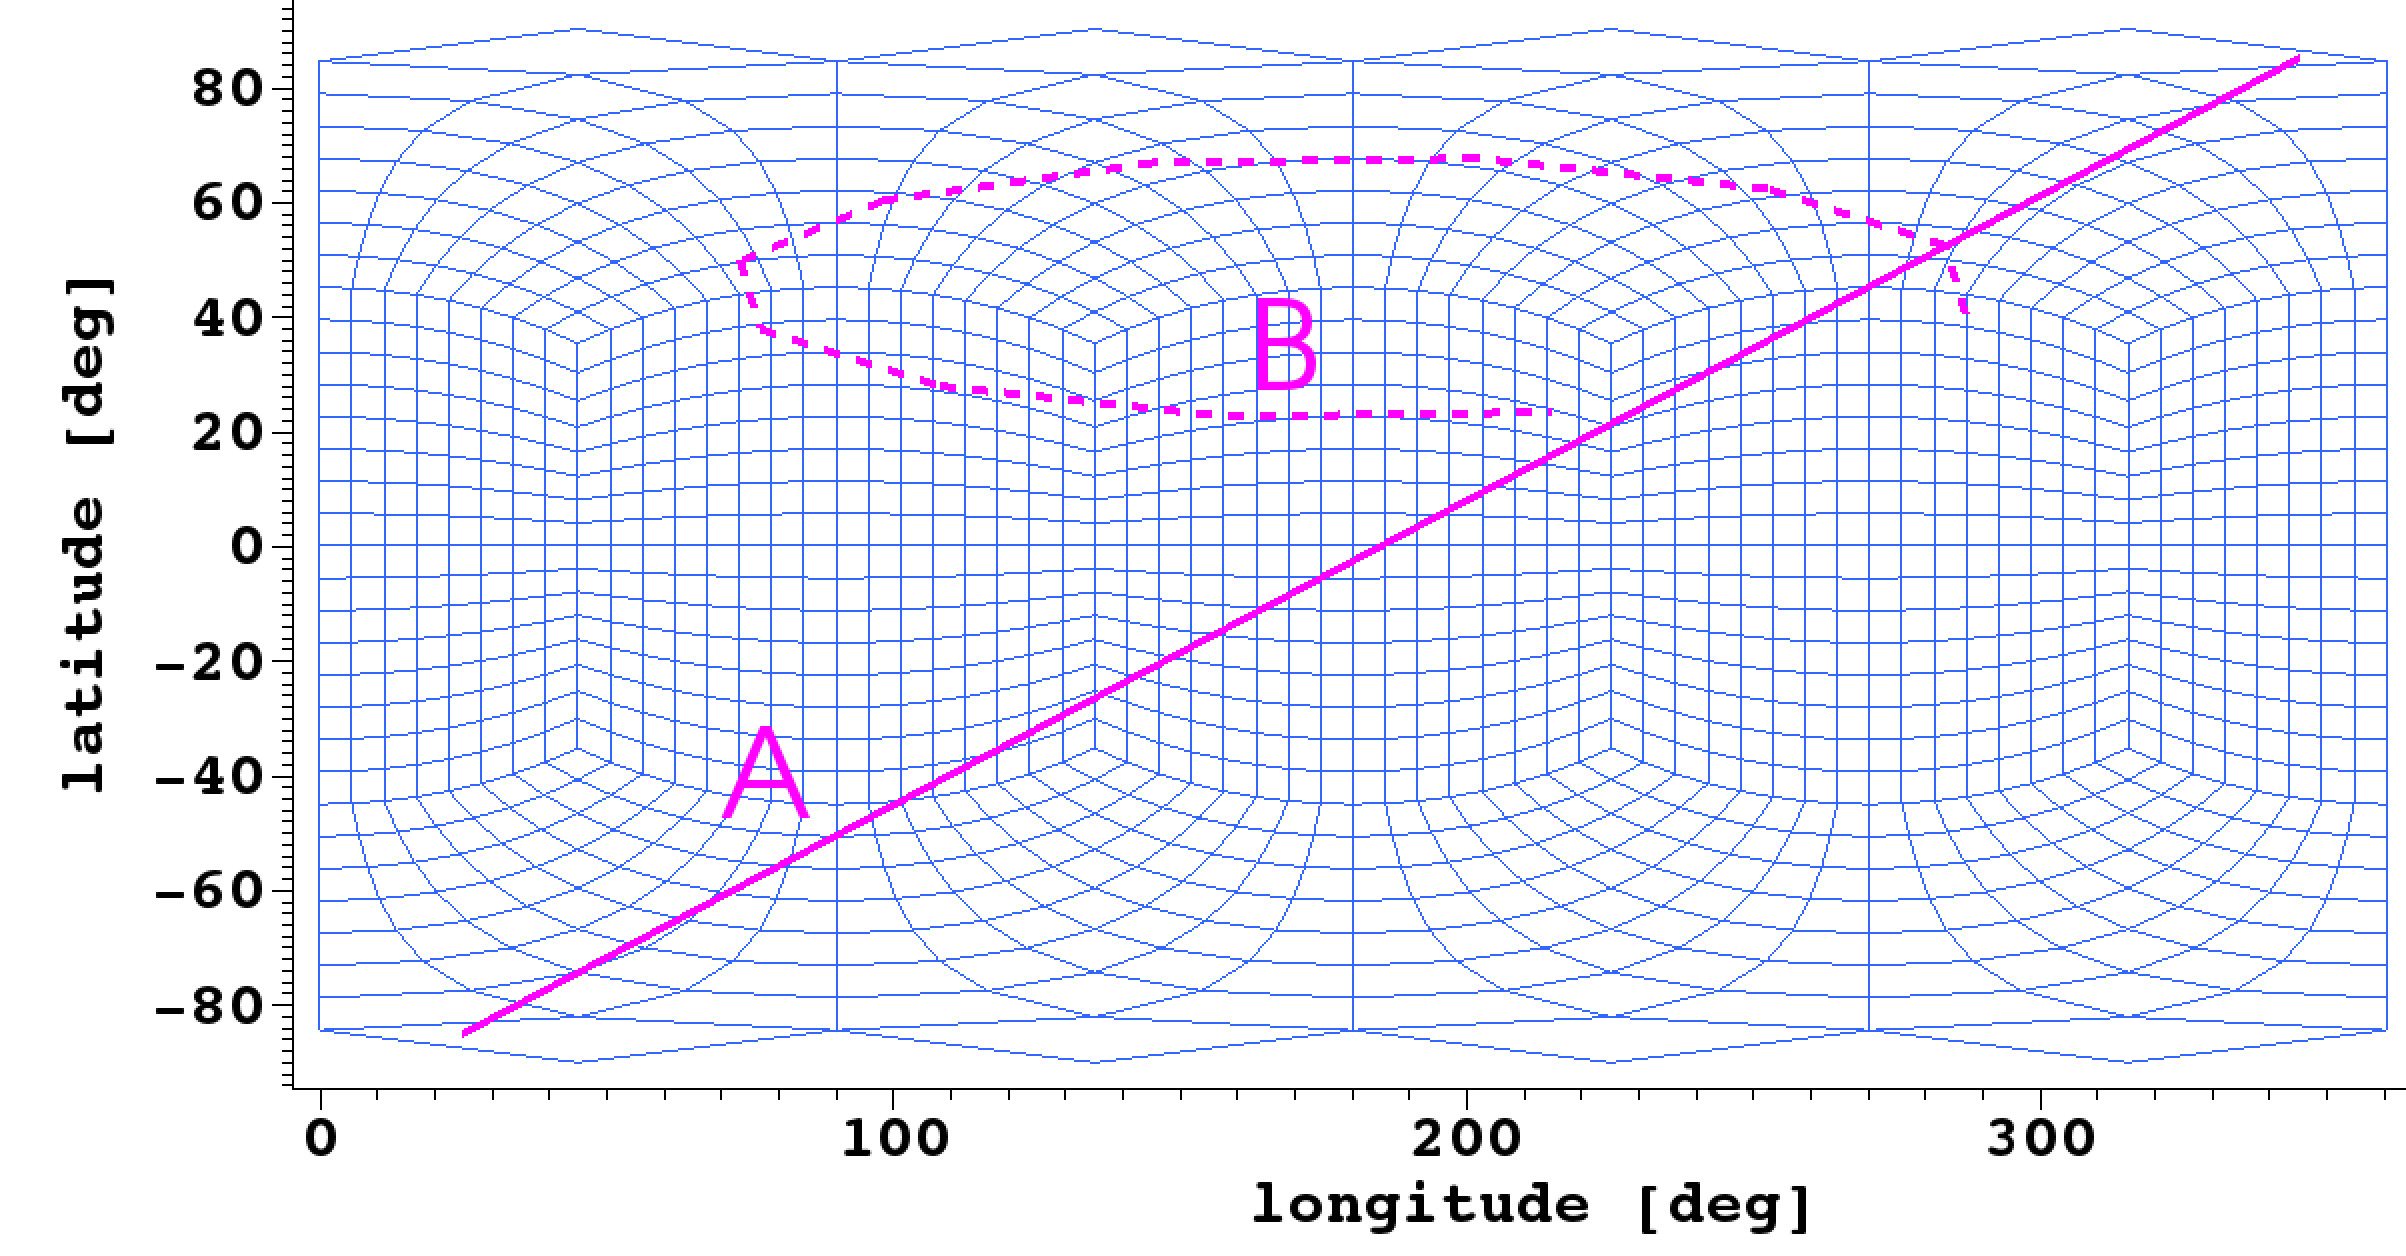
\includegraphics[width=75mm]{fluxOnCubedSphere.png} & 
  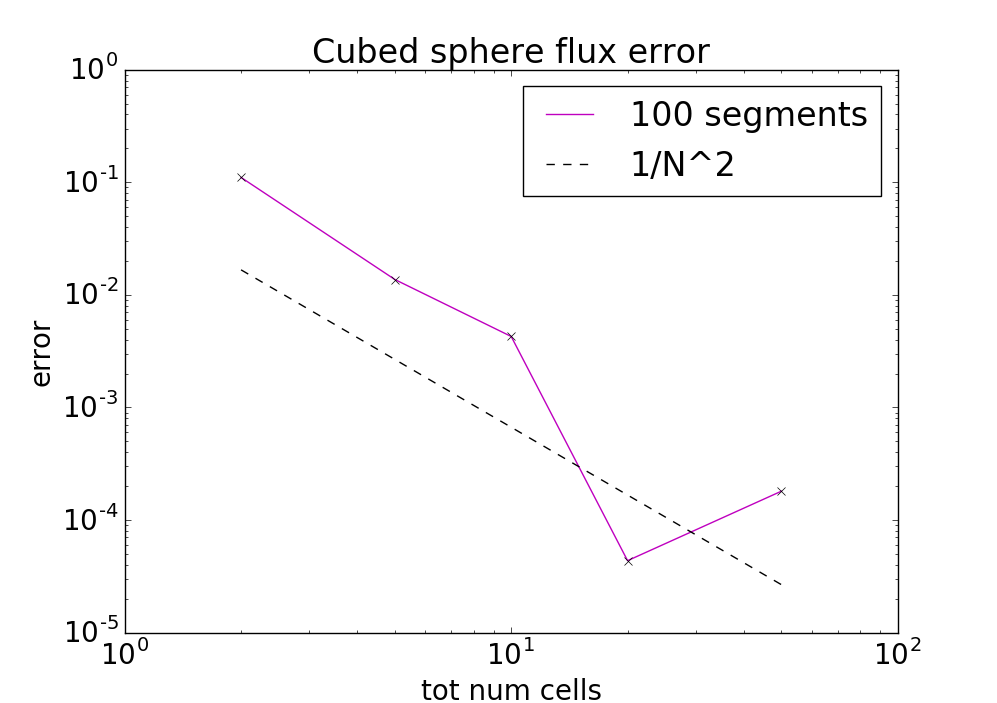
\includegraphics[width=60mm]{cubedSphereFluxError.png} \\
  {Integration path/surface} & {Error is $\sim 1/N^2$} 
  \end{tabular}
\end{frame}

\BackgroundPicture{NeSI/divider-02.png}
\begin{frame}[fragile]{}
  \begin{center}
    \Huge{\textbf{Summary}}
  \end{center}
\end{frame}
\BackgroundPicture{NeSI/blank-01.png}

\begin{frame}[t]
  \frametitle{}
    \begin{block}{Different types of field $\leftrightarrow$ different staggerings}
      \begin{itemize}%[<+-| alert@+>]
	  \item nodal for scalar fields (e.g. temperature)
	  \item edge for vector fields (e.g. electric field, velocity)
	  \item face for pseudo-vector fields (e.g velocity)
	  \item cell for pseudo-scalar fields (e.g. density)
	  \item type of field $\rightarrow$ interpolation method
      \item field values set via cell, face and edge integrals (instead of vector field components)
    \end{itemize}
    \end{block}
    \begin{block}{Masking and partially valid cells?}
	 Ok if taking account of partial cell, faces, edges when setting cell, face and edge integrals. Done!
  \end{block}
\end{frame}

\begin{frame}[t]
  \frametitle{Basis function extensions}
    \begin{block}{What about tetrahedra?}
      Similar approach except that the basis functions are Whitney's
    \end{block}
    \begin{block}{Higher order basis functions?}
    Initial work indicates that higher order basis functions can be used. These also satisfy the orthogonality condition $\int_i \phi_j = \delta_{ij}$
    on sub-cell edges, faces and cells. Quadratic elements effectively 
     split each cell into 8 sub-cells, each face into 4 sub-faces and each edge into 2 sub-edges. 
  \end{block}
\end{frame}

% End <-----------------------------------------------------------------------------------------
\BackgroundPicture{NeSI/blank-02.png}
\begin{frame}[plain]
  \begin{center}
  Goal is to apply the rigour of dynamical cores to pre- and post-processing tools. Overtime we expect the distinction between dynamical core
  and pre-/post-processing to diminish.
  \\
  
    \vspace*{+2cm}
    {\Huge Thank You}\\
    \vspace*{+1cm}
    
\includegraphics[width=100pt]{NeSI/nesi_logo.png}
  \end{center}
\end{frame}

\end{document} 